\section{Technology Stack}

The feature hypothesis (\autoref{sub:hypothesis}) states that networking,
persistence, serialization, session management and game engine integration are
necessary to build a fully functional \og{}. These essential features are
mandatory to drive an \og{}.

In addition to this core technology, supplementary technologies are needed to
help fulfill the deployment and the simple development hypothesis
(\autoref{sub:hypothesis}). These technologies are: Container engine,
composition engine, continuous integration solution, source control system, and
interactive development environment (IDE).

The rest of this section describes each technology and states advantages and
disadvantages along with the arguments which are decisive for the composition
of the technology stack.

\subsection{Core Technologies}

The core technologies have mostly been defined in the prior two project thesis.
This section gives a short summary on the chosen technology.

\subsubsection{Networking}

\begin{wrapfigure}{r}{4cm}
    
\includegraphics[width=4cm]{images/dependencies/activemq}
\end{wrapfigure}

\textbf{ActiveMQ} is a popular message broker. A message broker buffers
messages and delivers them as soon as a receiver is available. This allows for a
robust persistent messaging. Message brokers have been evaluated during
project thesis one. ActiveMQ is the networking foundation of MicroNet and
has proven to be very stable.

PostgreSQL is available on Docker Hub as a Docker image and can therefore
be integrated into a \ms{} application very easily using a composition engine.




\subsubsection{Persistence}

\begin{wrapfigure}{r}{4cm}
 	\hspace*{0.4cm}
    
\includegraphics[width=4cm]{images/dependencies/PostgreSQL}
\end{wrapfigure}

\textbf{PostgreSQL} is a very mature open source relational database. It is
available on all major platforms which allows for comfortable testing and
deployment. Since version 9.2 PostgreSQL supports the json data-type. This makes
it trivial to control the data flow from the network to the database.

PostgreSQL is also available on Docker hub and therefore allows quick
deployment. For production purposes a native installation of PostgreSQL is
suggested to provide the needed stability as explained in \todo{ref}.\\


\begin{wrapfigure}{r}{4cm}
    
\includegraphics[width=4cm]{images/dependencies/couchbase}
\end{wrapfigure}

\noindent
\textbf{Couchbase} is a NoSQL database realized as a Json document store. The
Json affinity of Couchbase integrates very well in the technology stack.
Couchbase has its own query language called N1QL which allows aggregated
querries between multiple documents. Also access on sub-document level is
possible to allow fine grained data access.

Couchbase can run in a cluster and maintains a quorum on document to provide
eventual consistency on writes which allows to scale the database system.
Couchbase also provides timeouts of documents which can be used to imitate
\textit{session store} behaviour. This neglects the need for a distributed
caching system like Redis for example. 

Even if Couchbase exists as a Docker image it is advised to install
Coutchbase native for production for the reasons explained in
\autoref{sub:database_solutions}.
    
\subsubsection{Serialization}

\begin{wrapfigure}{r}{4cm}
    
\includegraphics[width=4cm]{images/dependencies/google-gson}
\end{wrapfigure}

\textbf{Gson} from Google offers a very convenient out-of-the-box approach to
serialize Java objects to Json strings and vice versa. An advantage of Gson is that
also supports generic collections like hash-maps.

The main advantage of Gson is it's simplicity. The simplicity goes to the
cost of performance especially for the de-serialization of json strings.
Because of this reason simpel Json serialization is only usable is the
performance hit does not influence the application behaviour.

\subsubsection{Game Engine}

\begin{wrapfigure}{r}{4cm}
    
\includegraphics[width=4cm]{images/dependencies/Unity3D}
\end{wrapfigure}
    
Unity3D is very popular among independent developers because it has no
initial financial barrier. Unity is very well documented and has a very
healthy community to provide aid for development problems.

Unity3D provides a rich editor that allows to prototype games quickly. It
also offers a rich C\# API which allows to write any imaginable game logic. 

For this thesis it is in particular interesting how well the combination of
C\# game logic and Java back-end logic works in regards to the \ms{} tenet
polyglot programming.
    


\subsection{Supplementary Technologies}

The supplementary technologies have been under intense evaluation during this
thesis. The result of this evaluation is a set of technologies which work well
together, are easy to learn and are open source or have a community edition.

\subsubsection{Container Engine}

\begin{wrapfigure}{r}{4cm}
	\vspace*{-0.5cm} \hspace*{0.2cm}
    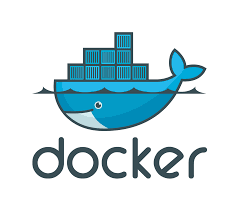
\includegraphics[width=3cm]{images/dependencies/docker}
\end{wrapfigure}

Docker has already been mentioned several times during this thesis. The
essence is that it all boils down to Docker being an enabler technology.
This is because all other technologies support Docker in some way. This
aspect makes the Docker Engine a reliable intermediate layer between the
actual hardware and the application that is running. 


\subsubsection{Composition Engine}

\begin{wrapfigure}{r}{4cm}
	\vspace*{-0.5cm} \hspace*{0.4cm}
    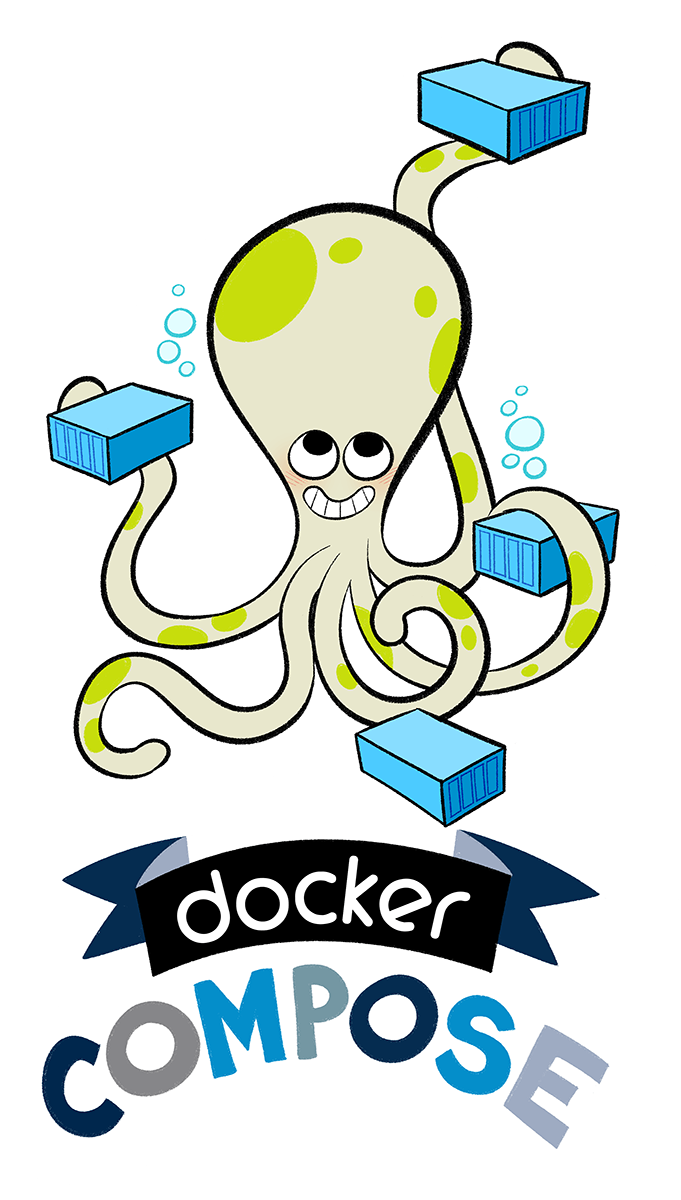
\includegraphics[width=2.4cm]{images/dependencies/docker-compose}
\end{wrapfigure}

Docker compose is basically only a CLI application which translates a
docker-compose file into a set of docker commands which are executed
sequentially. The result is a containerized application running on a single
host. Docker-compose is very helpful to quickly deploy a \ms{} application
stack locally. The docker-compose format also provides the basis to deploy a
composed application in the cloud using docker-swarm.\\

\newpage

\begin{wrapfigure}{r}{4cm}
    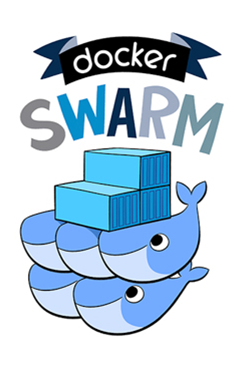
\includegraphics[width=4cm]{images/dependencies/docker-swarm}
\end{wrapfigure}

Docker-swarm allows to run containerized applications on a cluster of docker
machines. A docker machine is simply a host running a docker engine. Docker
swarm allows to set up application stack purely with docker commands or by
deploying a stack defined in a docker-compose file. Docker swarm offers
multiple scheduling strategies which distribute the containers among the
available docker machines.

The major advantage of docker-swarm is its simplicity. The set of command
needed to control the cluster is very limited and therefore very easy to
understand. Also since it is the native Docker composition technology it is
a natural match for Docker applications.

One noticable disadvantage is the lack of several convenience features like
a build-in dashboard or auto-scaling support. This is not a big concern
since many third party dashboard tools like Grafana are available and
auto-scaling can be added with a little implementation effort. 

\subsubsection{Continuous Integration}

Continuous integration is generally a party of every software project and \og{}
are no exception. The continuous integration process is developed to the point
where a central build system like Jenkins can unify the whole build process
but this aspect is not covered in this thesis.\\

\begin{wrapfigure}{r}{4cm}
    
\includegraphics[width=4cm]{images/dependencies/maven}
\end{wrapfigure}

Maven provides a convenient way to define the build process of Java
applications. For the game back-end services which are mainly written in Java
this is a perfect match to define the build process.

Maven also works very well in conjunction with Docker. The Maven Docker image
allows for easily integrate the Java build process into the Docker build
process by executing the Maven build inside the target container. This approach
removes the need of any local java or Maven installation. 

The drawback of the completely in-container Maven build is performance. Maven
downloads ``the whole Internet'' within the container to build the application.
This is not useful during development where short build times are mandatory. To
cope with this problem the maven build can be conducted on the host system and
only the binaries are send to the Docker daemon for the container build. This
makes the build much faster and has no real disadvantage because the process
can be reproduced exactly on the build system and therefor also speeds up
automated builds.

Maven is also very useful to preserve a consistent versioning of \mss{}. The
game application stack can be described using a master .pom file containing
current version of all services. The master .pom file can be updated to
introduce new versions of any service. The continuous integration process can
be triggered at this point to perform a rolling update with the currently
deployed application stack.\\
	
\begin{wrapfigure}{r}{4cm}
    
\includegraphics[width=4cm]{images/dependencies/github}
\end{wrapfigure}

Git is the \textbf{Source Control System} that builds the foundation for the
version control. Git allows to share Maven projects which in turn allows to
reproduce the build process locally but also on a build server. 

Github is used to provide any needed dependency used for the build process.
This includes the MicroNet framework.

\subsubsection{Interactive Development Environment (IDE)}

IDE is a wide term for a tool that simplifies the development process of a
software program. Usually it provides comprehensive tools that assist in writing
the source code of an application.\\

\begin{wrapfigure}{r}{4cm}
    
\includegraphics[width=4cm]{images/dependencies/eclipse}
\end{wrapfigure}

Eclipse provides a very solid foundation to develop Java projects. The plug-in
development environment of Eclipse allows to customize the development to an
arbitrary extent. This aspect is especially useful because in regards to \ms{}
development no specific tools are available to conduct the whole development
process of a \ms{} application from the IDE to the cloud.

Also Eclipse provides a number of very useful plug-ins which further ease the
\ms{} development process.

The \textbf{Docker Tools} for Eclipse are a visual explorer  for Docker images
and containers. It allows to quickly start, stop, build and remove containers
without having to bother with the console.

\textbf{Launch Groups} is a plug-in contributed by Eclipse CDT (C++ development
plug-in for Eclipse). It is very useful to directly run or debug multiple
applications at once. This allows to quickly bring up or terminate the whole
application stack for testing purposes. Although CDT is required for Launch
Groups it does not interfere with java development.































